\chapter{Алгоритм дифузії для розв'язання задачі стереобачення}

Другий розділ присвячено розв'язку задачі стереобачення алгоритмом дифузії.
Описуються властивості алгоритму та з'ясовується придатність
розв'язку для поставленої задачі.

\section{Алгоритм дифузії для розв'язання задачі стереобачення}

Алгоритм дифузії є блочно-координатним підйомом
\cite{overview:savchynskyy:diffusion}.
Кожній вершині графу $\left( x, y, d \right)$,
де $\left(x, y \right) \in T, \, d \in D$,
ставиться у відповідність блок змінних
$\left(
    \varphi_{\left(x, y \right), \left(x', y' \right)} \left(d \right) \in
    \mathbb{R} :
    \left(x', y' \right) \in \mathcal{N} \left(x, y \right), \,
    d \in D
\right)$ (рис.~\ref{fig:phi:block}).
Введені змінні будемо називати потенціалами.

\begin{figure}[h]
  \centering
  \includegraphics[width=0.6\textwidth]{images/phi_block}
  \caption{Змінна $\varphi_{\left(x, y \right), \left(x', y' \right)} \left(d \right)$}
  \label{fig:phi:block}
\end{figure}

Вводяться репараметризовані ваги вершин
(рис.~\ref{fig:reparametrized:vertex:weight})
\begin{equation} \label{reparametrized:vertex}
\begin{gathered}
    f_{\left(x, y \right)}^{\varphi} \left( d \right) :=
        f_{\left(x, y \right)} \left( d \right)
        - \sum \limits_{\left(x', y' \right) \in \mathcal{N} \left(x, y \right)}
            \varphi_{\left(x, y \right), \left(x', y' \right)} \left(
                d
                \right), \; \;
    \left(x, y \right) \in T, \; \;
    d \in D,
\end{gathered}
\end{equation}
тобто від вихідного штрафу в вершині віднімаються потенціали,
що виходять із даної вершини в усі сусідні об'єкти.

\begin{figure}[h]
  \centering
  \includegraphics[width=0.7\textwidth]{images/reparametrized_vertex_weight}
  \caption{Потенціали, які віднімаються від вихідного штрафу в вершині $\left(x, y, d \right)$}
  \label{fig:reparametrized:vertex:weight}
\end{figure}

Також вводяться репараметризовані ваги дужок (рис.~\ref{fig:reparametrized:edge:weight})
\begin{equation} \label{reparametrized:edge}
\begin{gathered}
    g_{\left(x, y \right), \left(x', y' \right)}^{\varphi} \left(d, d' \right)
    := g_{\left(x, y \right), \left(x', y' \right)} \left(d, d' \right)
    + \varphi_{\left(x, y \right), \left(x', y' \right)} \left(d \right)
    + \varphi_{\left(y', x' \right), \left(x, y \right)} \left(d' \right), \\
    \left(
        \left(x, y \right), \left(y', x' \right)
    \right) \in \mathcal{N}, \; \;
    d, d' \in D,
\end{gathered}
\end{equation}
тобто до вихідного штрафу в дужці додаються потенціали, що виходять в об'єкти,
які дана дужка поєднує.

\begin{figure}[h]
  \centering
  \includegraphics[width=0.6\textwidth]{images/reparametrized_edge_weight}
  \caption{Потенціали, які додаються до вихідного штрафу в дужці між вершиною
           $\left(x, y, d \right)$ та вершиною $\left(x', y', d' \right)$}
  \label{fig:reparametrized:edge:weight}
\end{figure}

Після перетворень \eqref{reparametrized:vertex} та \eqref{reparametrized:vertex}
значення штрафної функції не зміниться для будь-якої розмітки $\pmb{d} \in D^T$.
Для доведення цього твердження запишемо штрафну функцію
\eqref{eq:overview:penalty} з репараметризованими штрафами
\eqref{reparametrized:vertex} та \eqref{reparametrized:vertex}
\begin{equation*}
\begin{gathered}
    E^{\varphi} \left( \pmb{d} \right)
    = \sum \limits_{\left(x, y \right) \in T}
        f_{\left(x, y \right)}^{\varphi} \left(
            d \left(x, y \right)
        \right) + \\
    + \sum \limits_{\left(\left(x, y \right), \left(x', y'\right) \right) \in \mathcal{N}}
        g_{\left(x, y \right), \left(x', y' \right)}^{\varphi} \left(
            d \left( x, y \right), d \left( x', y' \right)
        \right) = \\
    = \sum \limits_{\left(x, y \right) \in T} \left[
        f_{\left(x, y \right)} \left( d \left(x, y \right) \right)
        - \sum \limits_{\left(x', y' \right) \in \mathcal{N} \left(x, y \right)}
            \varphi_{\left(x, y \right), \left(x', y' \right)} \left(
                d \left(x, y \right)
            \right)
        \right] + \\
        + \sum \limits_{\left(\left(x, y \right), \left(x', y'\right) \right) \in \mathcal{N}}
            \left[
                g_{\left(x, y \right), \left(x', y' \right)} \left(
                    d \left(x, y \right), d \left(x', y' \right)
                \right) + \right. \\
                \left.
                + \varphi_{\left(x, y \right), \left(x', y' \right)}
                    \left( d \left(x, y \right)
                \right)
                + \varphi_{\left(x', y' \right), \left(x, y \right)}
                    \left( d \left(x', y' \right)
                \right)
            \right].
\end{gathered}
\end{equation*}
Розкриємо дужки в останньому виразі
\begin{equation*}
\begin{gathered}
    E^{\varphi} \left( \pmb{d} \right)
    = \sum \limits_{\left(x, y \right) \in T}
        f_{\left(x, y \right)} \left(d \left(x, y \right) \right)
    - \sum \limits_{\left(x, y \right) \in T}
        \sum \limits_{\left(x', y' \right) \in \mathcal{N} \left(x, y \right)}
            \varphi_{\left(x, y \right), \left(x', y' \right)} \left(
                d \left(x, y \right)
            \right) + \\
    + \sum \limits_{\left( \left(x, y \right), \left( x', y' \right) \right) \in \mathcal{N}}
        g_{\left(x, y \right), \left(x', y' \right)} \left(
            d \left(x, y \right), d \left(x', y' \right)
        \right) + \\
    + \sum \limits_{\left( \left(x, y \right), \left( x', y' \right) \right) \in \mathcal{N}}
        \left[
            \varphi_{\left(x, y \right), \left(x', y' \right)} \left(
                d \left(x, y \right)
            \right)
            + \varphi_{\left(x', y' \right), \left(x, y \right)} \left(
                d \left(x', y' \right)
            \right)
        \right] = E \left(\pmb{d} \right),
\end{gathered}
\end{equation*}
адже перший та третій доданки дорівнюють $E \left( \pmb{d} \right)$,
а інші доданки разом дорівнюють нулю.
Отримали, що
$E^{\varphi} \left(\pmb{d} \right)
    = E \left(\pmb{d} \right)$
для всіх розміток $\pmb{d} \in D^T$.
Отже, репараметризовані ваги введено правильно.

Елементарний крок алгоритму дифузії
складається з двох операцій для кожного об'єкту $\left(y, x \right)$:
\begin{equation}\label{eq:diffusion:first}
\begin{gathered}
    \forall \left( y', x' \right) \in \mathcal{N} \left(y,x\right) \; \;
    \forall d \in D_x \\
    \varphi_{\left(y, x \right), \left(y', x' \right)}^{t + 1} \left( d \right)
    := \varphi_{\left(y, x \right), \left(y', x' \right)}^t \left( d \right)
    - \min \limits_{d' \in D_{x'}}
        g^{\varphi^t} \left(d, d' \right),
\end{gathered}
\end{equation}
\begin{equation}\label{eq:diffusion:second}
\begin{gathered}
    \forall \left( y', x' \right) \in \mathcal{N} \left(y,x\right) \; \;
    \forall d \in D_x \\
    \varphi_{\left(y, x \right), \left(y', x' \right)}^{t + 2} \left( d \right)
    := \varphi_{\left(y, x \right), \left(y', x' \right)}^{t + 1} \left( d \right)
    + \frac{f^{\varphi^{t + 1}} \left(L \left(y, x\right) , R \left(y, x - d\right)\right)}{\left| \mathcal{N} \left(y, x \right)\right|},
\end{gathered}
\end{equation}
де через $t$ позначено номер ітерації.

Для фіксованої вершини $\left( y, x, d \right)$ перша операція
\ref{eq:diffusion:first} знаходить мінімальну вагу дужки між заданою вершиною
та всіма вершинами $\left( y', x', d'\right)$,
де $d' \in D_{x'}$,
з сусідніх до неї об'єктів
$\left(y', x' \right) \in \mathcal{N} \left(y, x \right)$,
віднімає її від ваг усіх цих дужок
$\left( \left(y, x, d\right), \left( y', x', d'\right)\right)$
та додає до ваги вершини $\left(y, x, d \right)$.
В результаті мінімальна вага дужки між вершиною $\left( y, x, d \right)$
та кожним її сусідом $\left(y', x' \right) \in \mathcal{N} \left(y, x \right)$
дорівнює нулю.

Після цього друга операція \ref{eq:diffusion:second}
перерозподіляє репараметризовані ваги вершин
$f^{\varphi} \left(
    L \left(y, x \right) , R \left(y, x - d \right)
\right) $
між дужками до всіх сусідніх об'єктів
$\left(y', x' \right) \in \mathcal{N} \left(y, x \right)$.
В результаті вага вершини $ \left( y, x, d \right)$ стає рівною нулю,
а мінімальні ваги дужок з цієї вершини до всіх сусідніх об'єктів стають
рівними одна одній.

Іншими словами, після операцій \ref{eq:diffusion:first} і
\ref{eq:diffusion:second} для об'єкта $\left(y, x \right) \in T$ виконується
\begin{equation*}
    f^{\varphi} \left(
        L \left(y, x\right) , R \left(y, x - d \right)
    \right) = 0, \; \; \forall d \in D_x,
\end{equation*}
\begin{equation*}
    \min \limits_{d' \in D_{x'}} g \left( d, d' \right)
    = \min \limits_{d'' \in D_{x''}} g \left( d, d'' \right), \; \;
    \forall \left(y', x' \right), \,
        \left(y'', x'' \right) \in \mathcal{N} \left(y, x \right), \; \;
    d \in D_x.
\end{equation*}

% TODO: add image for illustration of elementary diffusion step (probably, from book)

Відомо \cite{overview:savchynskyy:diffusion},
що операції \ref{eq:diffusion:first} і
\ref{eq:diffusion:second} максимізують двоїсту функцію Лагранжа за змінними
$\left(
    \varphi_{\left(y, x \right), \left(y', x' \right)} \left(d \right) :
    \left(y', x' \right) \in \mathcal{N} \left(y, x \right), \,
    d \in D_x
\right)$, а тому мінімізують штрафну функцію \ref{eq:overview:penalty}.

Алгоритм полягає в ітеративному повторі елементарного кроку дифузії до виконання
критерію зупинки.

На першій ітерації вважається, що
$\varphi_{\left(y, x \right), \left(y', x' \right)} \left(d \right) = 0$
для всіх об'єктів $\left(y, x \right) \in T$, всіх міток $d \in D_x$
та всіх сусідніх об'єктів
$\left(y', x' \right) \in \mathcal{N} \left(y, x \right)$.

\section{Вибір найкращої розмітки}

% TODO: cite crossing out algorithm

Після завершення якоїсь кількості ітерацій алгоритму дифузії,
перевіряється, чи досягається необхідна точність за допомогою
алгоритма викреслювання другого порядку.
На вже побудованому графі розв'язується
$\left( \bigvee, \bigwedge \right)$-задача.

% TODO: use ampersand notation

Тепер кожна вершина і дужка графу може бути допустимою або ні.
$\tilde{f}_{\left(y, x \right)} \left(d \right) \in \left\{ 0, 1 \right\}$
означає допустимість мітки
$d \in D_x$ в об'єкті $\left(y,x \right) \in T$.
Аналогічно,
$\tilde{g}_{\left(y,x \right), \left(y', x' \right)} \left(d, d' \right)
    \in \left\{ 0, 1 \right\}$
означає допустимість пари міток $d \in D_x$ і $d' \in D_{x'}$
в парі сусідніх об'єктів
$\left( \left(y,x \right), \left(y', x' \right) \right) \in \mathcal{N}$.

На початку всі вершини вважаються допустимими, тобто
$\tilde{f}_{\left(y, x \right)} \left(d \right) = 1$ для всіх
міток $d \in D_x$ в об'єкті $\left(y,x \right) \in T$.
В кожній парі сусідніх об'єктів знаходиться дужка з мінімальною вагою.
Між цією парою об'єктів допустимими є ті дужки,
вага яких відрізняється від мінімальної не більше
наперед заданої малої величини $\varepsilon$.

Алгоритм полягає в багатократному застосуванні операцій
<<викреслювання вершини>>
\begin{equation*}
    \tilde{f}_{\left(y, x \right)} \left(d \right)
    := \tilde{f}_{\left(y, x \right)} \left(d \right)
    \bigwedge \bigwedge \limits_{\left(y', x' \right)\in \mathcal{N}\left(y,x \right)}
        \bigvee \limits_{d' \in D_{x'}}
            \tilde{g}_{\left(y,x \right), \left(y', x' \right)}
                \left(d, d' \right)
\end{equation*}
та <<викреслювання дужки>>
\begin{equation*}
    \tilde{g}_{\left(y,x \right), \left(y', x' \right)} \left(d, d' \right)
    := \tilde{g}_{\left(y,x \right), \left(y', x' \right)} \left(d, d' \right)
    \bigwedge \tilde{f}_{\left(y, x \right)} \left(d \right)
    \bigwedge \tilde{f}_{\left(y', x' \right)} \left(d' \right).
\end{equation*}

% TODO: images for vertex and edge crossing out

Алгоритм завершує роботу зі скінченну кількість ітерацій.
Якщо після завершення роботи алгоритма деякі вершини залишились невикресленими,
то було зроблено досить ітерацій дифузії,
і з множини невикреслених вершин можна побудувати розмітку.
Інакше треба продовжити ітерації дифузії.

% TODO: cite this  property

Для гарантії збіжності алгоритму дифузії ваги дужок $g$
вихідного графу повинні мати властивість супермодулярності
\cite{diffusion:shlezinger:supermodularity}.
Прикладом вагової функції для дужок з властивістю супермодулярності є
\begin{equation*}
    g \left( d \left( y, x \right), d \left( y', x' \right) \right)
    = \left| d \left( y, x \right) - d \left( y', x' \right) \right|.
\end{equation*}

% TODO: image for illustration of supermodularity
% TODO: term consistency: вагова or штрафна функція

\section*{Висновки до розділу 2}
\addcontentsline{toc}{section}{Висновки до розділу 2}

Пред'явлено розв'язок задачі стереобачення за допомогою алгоритма дифузії.
За певних штрафних функцій алгоритм гарантовано збігається,
проте на практиці алгоритм працює досить довго, а отже потребує оптимізації.
